% sezione dedicata al preambolo.
\documentclass[12pt,a4paper]{article}
\usepackage[T1]{fontenc}
\usepackage[utf8]{inputenc}
\usepackage[italian]{babel}
\usepackage{tabularx}
\usepackage{booktabs}
\usepackage{float}
\usepackage{caption}
\captionsetup{tableposition=top,figureposition=bottom,font=small}
\usepackage{graphicx}
\usepackage{listings}
\usepackage{color}
\usepackage{amsmath}
\usepackage{fancyhdr}

\definecolor{codegreen}{rgb}{0,0.6,0}
\definecolor{codegray}{rgb}{0.5,0.5,0.5}
\definecolor{codepurple}{rgb}{0.58,0,0.82}
\definecolor{backcolour}{rgb}{0.95,0.95,0.92}

\lstdefinestyle{mystyle}{
    backgroundcolor=\color{backcolour},
    commentstyle=\color{codegreen},
    keywordstyle=\color{magenta},
    numberstyle=\tiny\color{codegray},
    stringstyle=\color{codepurple},
    basicstyle=\scriptsize,
    breakatwhitespace=false,
    breaklines=true,
    captionpos=b,
    keepspaces=true,
    numbers=left,
    numbersep=5pt,
    showspaces=false,
    showstringspaces=false,
    showtabs=false,
    tabsize=2,
    xleftmargin=0.03\textwidth,
    xrightmargin=0.03\textwidth
}

\lstset{style=mystyle}

\newcommand*{\plogo}{\fbox{$\mathcal{PL}$}} % Generic publisher logo

%----------------------------------------------------------------------------------------
%   TITLE PAGE
%----------------------------------------------------------------------------------------

\newcommand*{\titleGP}{\begingroup % Create the command for including the title page in the document
\centering % Center all text
\vspace*{\baselineskip} % White space at the top of the page

\rule{\textwidth}{1.6pt}\vspace*{-\baselineskip}\vspace*{2pt} % Thick horizontal line
\rule{\textwidth}{0.4pt}\\[\baselineskip] % Thin horizontal line

{\LARGE BASI DI DATI\\ E \\[0.3\baselineskip] CONOSCENZA}\\[0.2\baselineskip] % Title

\rule{\textwidth}{0.4pt}\vspace*{-\baselineskip}\vspace{3.2pt} % Thin horizontal line
\rule{\textwidth}{1.6pt}\\[\baselineskip] % Thick horizontal line

\scshape % Small caps
Relazione della progettazione di una base di dati\\
relazionale per una competizione di Crossfit\\
[\baselineskip] % Tagline(s) or further description
Anno Accademico, 2015-2016\par % Location and year

\vspace*{2\baselineskip} % Whitespace between location/year and editors

Realizzato da \\[\baselineskip]
{\Large Roberto Pallotta\par} % Editor list
{\itshape Universita degli studi di Roma \\ Tor Vergata.\par} % Editor affiliation

\vfill % Whitespace between editor names and publisher logo

\endgroup}

% Available document structure commands:
% Article: \part{}, \section{}, \subsection{}, \subsubsection{}, \paragraph{}, \subparagraph{}.
\begin{document}
\titleGP
\newpage
\tableofcontents
\listoffigures
\newpage
\pagestyle{fancy}
\lhead{}
\chead{}
\renewcommand{\headrulewidth}{0.4pt}
\renewcommand{\footrulewidth}{0.4pt}
\section{Descrizione del progetto}

Il progetto scelto si prefige di realizzare una base di dati per una competizione di crossfit.
Il crossfit,nasce da Greg Glassman negli Stati Uniti all' inizio anni 70. Questa disciplina iniziò a diventare
popolare negli anni 90. Nel 1995 nacque la prima palestra box che si trovava a Santa Cruz in California.
Il Crossfit è un programma di rafforzamento e condizionamento fisico, pensato per aiutare le persone a conquistare un benessere completo e generale. Tale programma si concentra su una serie di movimenti funzionali che cambiano costantemente, eseguiti ad alta intensità, per raggiungere una prestanza fisica totale e rendere le persone pronte a ogni genere di sfida fisica.
Per una copetizione di crossfit bisogna avere a disposizione diverse palestre o box.
Un box è una palestra dedicata a chi svolge il Crossfit. La differenza tra una palestra e un box si trova nella struttura stessa,in un box si devono avere degli spazi liberi, dove i diversi gruppi possono eseguire esercizi a corpo libero, mentre in una palestra troviamo diversi macchinari che oltre a ridurre lo spazio sono non idonei per gli esercizi di crossfit.
In una palestra in genere si allenano diverse persone contemporaneamente, ma con un programma di allenamento totalmente differente tra loro. Nel box gli allenamenti si svolgono tra più gruppi di persone,le quali svolgono lo stesso tipo di allenamento,supervisionati da uno o più Coach.
In una competizione di Crossfit siamo in presenza di atleti, che devono essere maggiorenni e in ottima salute per poter partecipare. Un'altra fondamentale caratteristica presente nelle competizioni di crossfit è data dalla partecipazione di atleti in Team. Un Team è composto da un numero variabile di persone, e contiene uno o più Coach. Un Team, per sostenere le spese economiche necessarie alla competizione si avvale di più sponsor che li supportano economicamente. I team come già accennato possiedono uno o più Coach, i quali devono essere in possesso di una o più certificicazioni per poter essere definiti Coach. Le certificazioni,sono suddivise in quattro livelli differenti, ogniuno identificato da un codice. La competizione prevede che un Team esegua ,un wod,nel box dove sarà valutato da un giudice che gli assegnerà un punteggio compreso tra 0 e 100. Il wod consiste in una lista di esercizi che il team deve eseguire per poter essere valutato. Un wod possiede una data di pubblicazione e una data di termine,entro il quale il team deve completare il wod. La mancata esecuzione di un wod, non determinerà l'esclusione del team dalla competizione, ma solo la conquista di un minor punteggio, utile per il raggiungimento del risultato finale. Un wod deve essere esguito  esclusivamente nel box ad esso associato. Questo darà modo ai diversi team ospitati,di apprezzare le diverse tecniche di allenamento utilizzate in diverse località del mondo. Gli esercizi presenti nel wod devono essere compresi da tutti i Team, per questo motivo si dovrà disporre di una lista di esercizi con una berve descrizione funzionale. Per quanto riguarda quegli esercizi che comprendono un carico specifico, si devono rispettare determinati vincoli variabili per ogni tipo di attrezzo a seconda degli standard. In ogni competizione si avrà un pubblico. Volendo si potranno memorizzare i dati anagrafici di ogni persona che ha partecipato da spettatore,e si potrà memorizzare in quale box ha fatto da spettatore, per consentire l'uilizzo dei dati da perte dei box per fini statistici. Al termine della competizione sarà decretato il vincitore valutando i risultati ottenuti dai singoli team, per ogni wod, ottenendo una classifica generale.
\newpage
\section{Analisi dei requisiti}

L'analisi dei requisiti è sicuramente la fase fondamentale per la realizzazione di una base di dati. In questa sezione si raccolgono tutti quei concetti necessari a identificare le entità, e le relazioni che faranno parte dello schema Entity-Relationship. Le informazioni raccolte saranno divise in due tabelle, una per le entità e una per le relazioni.


\begin{table}[H]
\scriptsize
\centering
\caption[Entità]{Tabella delle entità con le relative descrizioni.}
\begin{tabularx}{\textwidth}{lXXl}
\toprule
Entità & Descrizione & Attributi & Identificatore \\
\midrule
\textbf{Atleta} & Una persona che partecipa alla competizione & E-mail,Nome,Cognome,Data di nascita,Sesso & E-mail \\
\midrule
\textbf{Coach} & Una persona che allena un determinato team & E-mail,Nome,Cognome,Data di nascita,Sesso & E-mail \\
\midrule
\textbf{Sponsor} & Un'azienda di vario tipo che sponsorizza il team supportandolo economicamente & Nome,Quota versata & Nome \\
\midrule
\textbf{Certificazione} & Attesta il grado di preparazione di un Coach & Id-livello,Descrizione & Id-livello \\
\midrule
\textbf{Team} & Identifica un insieme di Atleti ai quali si assegnano delle proprietà & Nome-team,Data-iscrizione,Stato & Nome-team\\
\midrule
\textbf{Wod} & Raccoglie un insieme di esercizi al quale viene assegnato un nome una data di pubblicazione e scadenza & Id-wod,Data-pubblicazione,Data-termine & Id-wod\\
\midrule
\textbf{Box} & Una palestra che si trova in un determinato stato & Nome-box,Stato & Nome-box\\
\midrule
\textbf{Giudice} & Identifica una persona che svolgerà il compito di giudice in una competizione & Id-giudice,Nome,Cognome,Data di nascita,Sesso & Id-giudice\\
\midrule
\textbf{Esercizio} & Descrive un componente del wod che un atleta deve eseguire in una competizione & Nome-esercizio,Descrizione & Nome-esercizio\\
\midrule
\textbf{Persona} & Una persona che farà da pubblico in una o più competizioni & Codice-fiscale,Nome,Cognome,Data di nascita,Sesso & Codice-fiscale\\
\bottomrule
\end{tabularx}
\end{table}

\begin{table}[H]
\scriptsize
\centering
\caption[Entità]{Tabella delle relazioni con le relative descrizioni.}
\begin{tabularx}{\textwidth}{lXXl}
\toprule
Relazione & Descrizione & Entità Coinvolte & Attributi \\
\midrule
\textbf{SP\_TE} & Associa uno sponsor a un team & Sponsor (0,1),Team (1,N) &  \\
\midrule
\textbf{AT\_TE} & Afferisce un atleta a un team & Atleta (1,1), Team (1,N) & \\
\midrule
\textbf{CO\_TE} & Associa a un team uno o più coach & Coach (1,1), Team (1,N) & \\
\midrule
\textbf{CO\_CE} & Associa una o più certificazioni a un coach & Coach (1,N), Certificazione (1,N) & \\
\midrule
\textbf{TE\_GI\_WO} & Mette in relazione un team un giudice e un wod per rappresentare una competizione & Team (1,N), Giudice (1,N), Wod (0,N) & Data esecuzione, Punteggio \\
\midrule
\textbf{WO\_ES} & Determina la composizione di un wod associando a esso uno o più esercizi & Wod (1,N), Esercizio (1,N) & \\
\midrule
\textbf{BO\_PE} & Associa una persona a uno o più box per rappresentare l'insieme degli spettatori & Box (0,N), Persona (0,N) & Data presenza \\
\bottomrule
\end{tabularx}
\end{table}

\newpage
\section{Regole Aziendali}
In questa sezione andremo a definire quelle regole che, nella terminologia delle basi di dati relazionali vanno sotto il nome di Regola di Vincolo, e Regola di Derivazione. Queste regole sono molto importanti se si vuole esprimere qualcosa che non può esser espressa tramite lo schema Entity-Relationship.

\subsection{Regole di Vincolo}
Una regola di vincolo può essere formulata utilizzando il linguaggio naturale, formulando delle asserzioni espresse nella forma dichiarativa.
\begin{description}
% 	struttura regole di vincolo < concetto > deve/ non deve < espressione su concetti >
	\item[RV1] Un atleta deve essere maggiorenne
	\item[RV2] Un coach deve essere maggiorenne
	\item[RV3] Un giudice deve essere maggiorenne
\end{description}

\subsection{Regole di Derivazione}
Le regole di derivazione possono essere espresse specificando le operazioni (aritmetiche o di altro genere) che permettono di ottenere il concetto derivato.
\begin{description}
	\item[RD1] L'età di un atleta,coach,giudice si ottiene effettuando una differenza tra la data corrente e la data di nascita.
	\item[RD2] Il punteggio finale ottenuto da un team si ottiene effettuando la somma di tutti i punteggi assegnati nei wod eseguiti meno il numero di wod non eseguiti.
\end{description}
\section{Schema Entity-Relationship}
Qui si riporta lo schema Entity-Relationship che descrive la base di dati che si vuole realizare tramite i costrutti forniti dal modello.
\begin{figure}
	\centering
	\caption[Entity Relationship]{Schema Entity-Relationship.}
	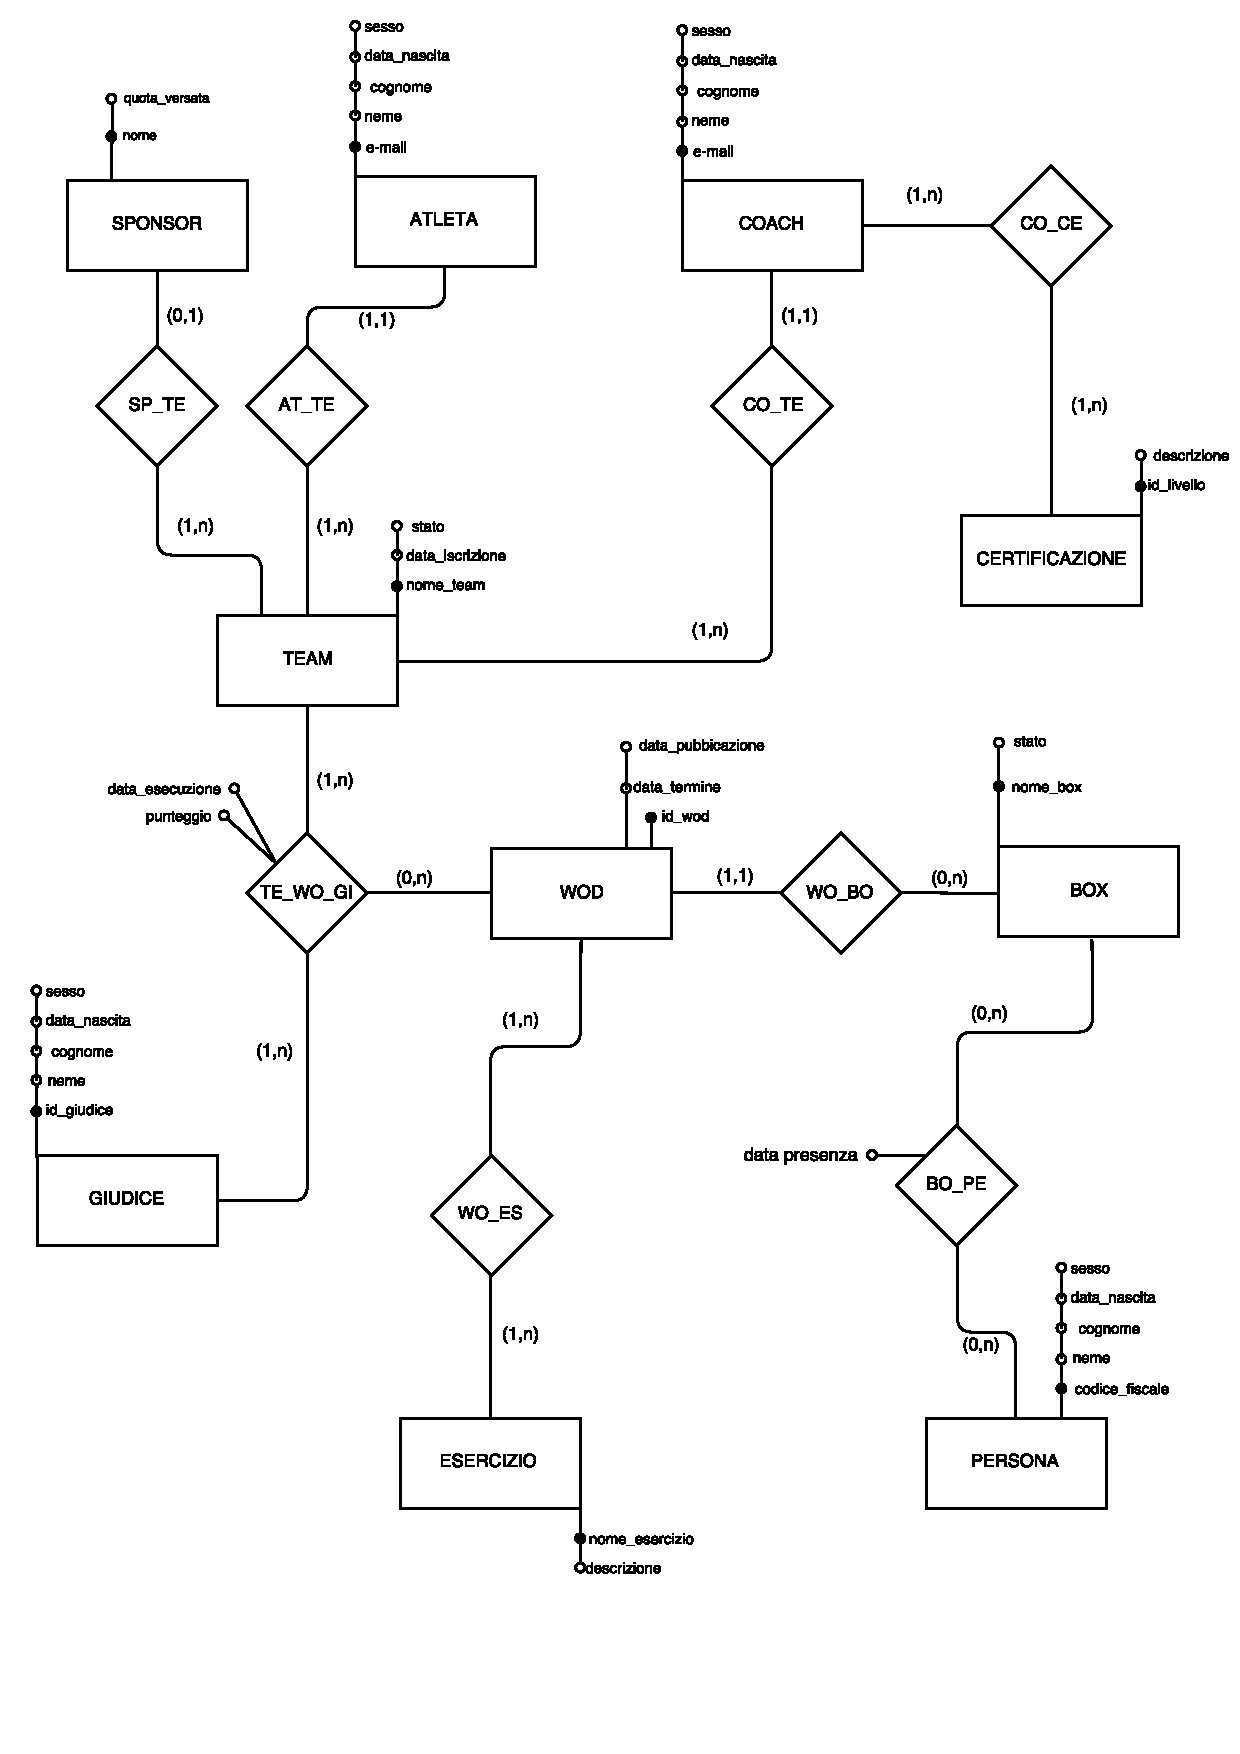
\includegraphics[width=\textwidth]{schemaer}
\end{figure}
\newpage
Normalmente si utilizza una modellazione che comprende tutti i costrutti necessari a rappresentare una base di dati relazionale, ma nella figura successiva possiamo vedere grazie al linguaggio UML (Unified Model Language) come possiamo modellare una base di dati relazionale grazie ai costrutti messi a disposizione da questo linguaggio. L'UML è fortemente utilizzato dall'ingegneria del software per modellare la struttura di un software grazie a un insieme di modelli messi a disposizione dal linguaggio. Nel modellare la base di dati con l'UML si è utilizzato il Class Diagram che normalmente è utilizzato per dare una visione statica degli oggetti che fanno parte di un software.
\begin{figure}
    \centering
    \caption[Entity Relationship UMLumlschemaer]{Schema Entity-Relationship con UML.}
    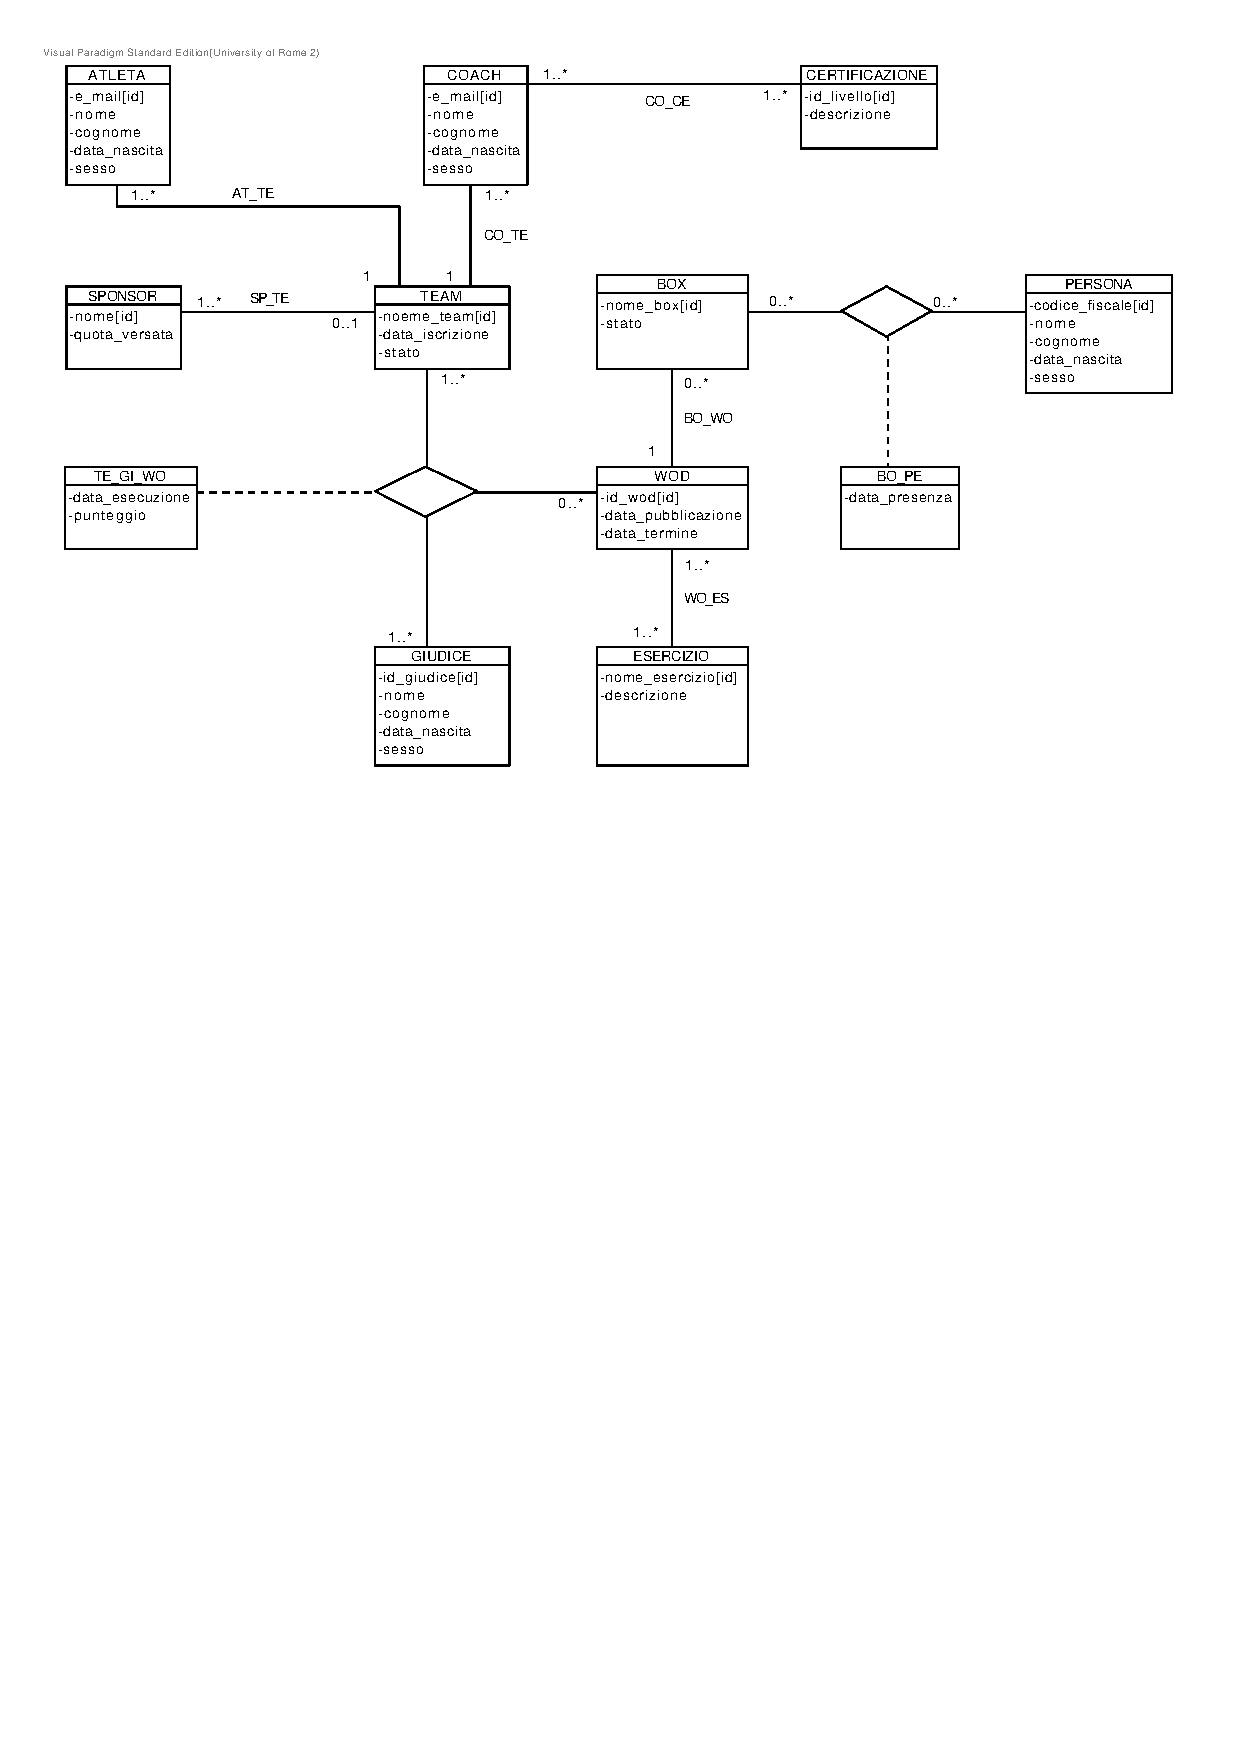
\includegraphics[width=\textwidth]{umlschemaer}
\end{figure}
\newpage
\section{Normalizzazione schema Entity-Relationship}
\subsection{Prima forma normale.}
Lo schema si presenta nella prima forma normale dato che tutti gli attributi sono in forma semplice, ovvero indivisibili.
\subsection{Seconda Forma Normale}
Uno schema è nella seconda forma normale, se è in prima forma normale, e tutti gli attributi di uno schema $R(X)$ sono totalmente dipendenti dalla chiave di $R(X)$. Nel caso dello schema presentato ci troviamo in questa situazione. Questo ci permette di affermare che la seconda forma normale è soddisfatta.
\subsection{Terza Forma Normale}
Lo schema si trova nella terza forma normale dato che ogni attributo che non fa parte della chiave di $R(X)$ è dipendente in modo non transitivo da ogni chiave.

\section{Schema Fisico}
Qui si presenta lo schema fisico ottenuto dallo schema Entity-Relationship dopo che si è verificato che questo sia nella terza forma normale. Questo schema risulta essere l'ultimo step nella fase progettuale della base di dati,prima che questa prenda vita in un DBMS vero e proprio.
\begin{figure}
	\centering
	\caption[Schema Fisico]{Schema Fisico.}
	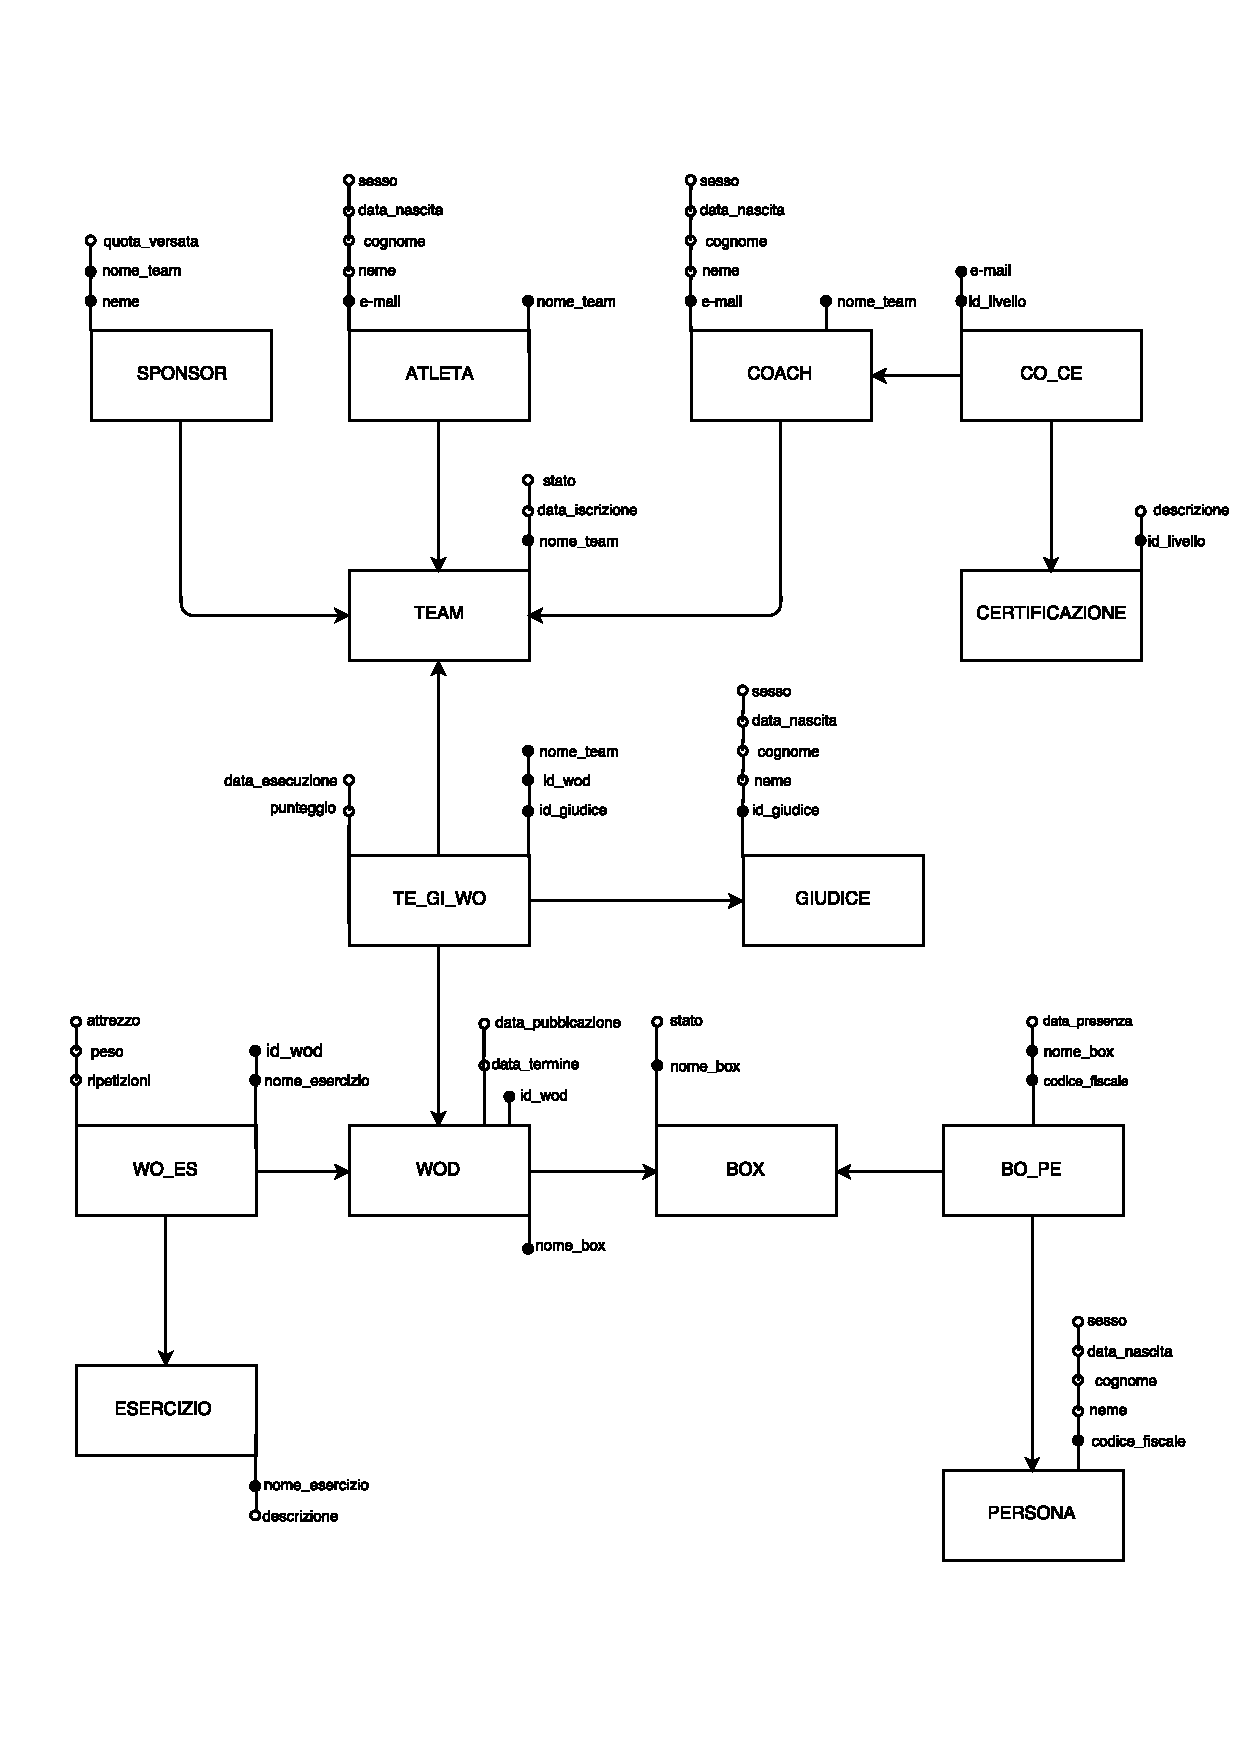
\includegraphics[width=\textwidth]{schemafisico}
\end{figure}
\newpage
\section{Creazione delle Entità e delle Relazioni.}
Questa parte del progetto mostra gli statements DDL (Data Definition Language). Il DDL è un sottoinsie del linguaggio SQL che permette di codificare le Entità e le Relazioni presenti nello schema fisico. Il DBMS scelto per realizzare la base di dati è MySQL di Oracle versione 5.6.27.
\lstinputlisting[language=SQL]{creadb.sql}

\newpage
\section{Inserimento dei dati nel database}
Si inseriscono dei dati di prova nel database utilizzando gli statements DML (Data Manipulation Language). Il DML è un sottoinsieme del linguaggio SQL.
\lstinputlisting[language=SQL]{insertdata.sql}

\newpage
\section{Query}
In questa sezione si elencano diverse query d'interesse relative alla base di dati che è stata realizzata precedentemente.

\subsection{Query 1}
\lstinputlisting[language=SQL,firstline=1,lastline=13]{query.sql}
\subsection{Query 2}
\lstinputlisting[language=SQL,firstline=15,lastline=20]{query.sql}
\subsection{Query 3}
\lstinputlisting[language=SQL,firstline=22,lastline=27]{query.sql}
\newpage
\subsection{Query 4}
\lstinputlisting[language=SQL,firstline=29,lastline=40]{query.sql}
\subsection{Query 5}
\lstinputlisting[language=SQL,firstline=42,lastline=51]{query.sql}
\subsection{Query 6}
\lstinputlisting[language=SQL,firstline=53,lastline=58]{query.sql}
\newpage
\subsection{Query 7}
\lstinputlisting[language=SQL,firstline=60,lastline=69]{query.sql}
\subsection{Query 8}
\lstinputlisting[language=SQL,firstline=71,lastline=79]{query.sql}
\subsection{Query 9}
\lstinputlisting[language=SQL,firstline=81,lastline=91]{query.sql}
\newpage
\subsection{Query 10}
\lstinputlisting[language=SQL,firstline=93,lastline=103]{query.sql}
\subsection{Query 11}
\lstinputlisting[language=SQL,firstline=105,lastline=114]{query.sql}
\subsection{Query 12}
\lstinputlisting[language=SQL,firstline=116,lastline=131]{query.sql}
\subsection{Query 13}
\lstinputlisting[language=SQL,firstline=133,lastline=140]{query.sql}
\subsection{Query 14}
\lstinputlisting[language=SQL,firstline=142,lastline=156]{query.sql}
\subsection{Query 15}
\lstinputlisting[language=SQL,firstline=158,lastline=169]{query.sql}
\newpage
\subsection{Query 16}
\lstinputlisting[language=SQL,firstline=171,lastline=180]{query.sql}
\subsection{Query 17}
\lstinputlisting[language=SQL,firstline=182,lastline=188]{query.sql}
\subsection{Query 18}
\lstinputlisting[language=SQL,firstline=190,lastline=197]{query.sql}
\newpage
\section{Algebra Relazionale}
In questa sezione si utilizzerà l'algebra relazionale per rappresentare alcune query che precedentemente sono state presentate in SQL.
\subsection{Query 1 in Algebra relazionale}
Nella prima query abbiamo utilizzato l'entità COACH e la relazione CO\_CE che sono rappresentate nello schema Entity Relationship, mentre le identifichiamo come entità fisiche nello Schema Fisico.

\begin{equation}
\begin{split}
    \pi_{nome,cognome,livello1,livello2,livello3,livello4}(\rho_{livello1 \leftarrow id\_livello}(CO\_CE) \\ \bowtie \rho_{livello2 \leftarrow id\_livello}(CO\_CE) \bowtie \\ \rho_{livello3 \leftarrow id\_livello}(CO\_CE) \bowtie \rho_{livello4 \leftarrow id\_livello}(CO\_CE))
\end{split}
\end{equation}

\subsection{Query 2 in Algebra Relazionale}
La seconda query, utilizza solo l'entità COACH per recuperare i dati che si vogliono ottenere. In Algebra relazionale possiamo ottenere lo stesso risultato come riportato di seguito.
\begin{equation}
\begin{split}
    \pi_{nome,cognome,sesso}(\sigma_{nome\_team='team01'}(COACH))
\end{split}
\end{equation}
\newpage
\section{Calcolo Relazionale}
Nella sezione riguardante l'Algebra Relazionale, abbiamo visto come trasformare le prime due query SQL in algebra relazinale. Ora vogliamo esprimere sempre le prime due query SQL in Calcolo Relazionale. Di seguito sono riportate le trasformazioni delle query.
\subsection{Query 1 in Calcolo Relazionale}
In questa query utilizziamo due schemi di relazione per ottenere i dati che si ottengono con la query SQL.
\begin{equation}
\begin{split}
\{nome:n,cognome:c,id\_livello:l1,\\id\_livello:l2, id\_livello:l3,id\_livello:l4 | \\ COACH(COACH(e\_mail:e,nome:n,cognome:c) \\ \land CO\_CE(e\_mail:e,id\_livello:l1)) \\ \land CO\_CE(e\_mail:e,id\_livello:l2)) \\ \land CO\_CE(e\_mail:e,id\_livello:l3)) \\ \land CO\_CE(e\_mail:e,id\_livello:l4)) \}
\end{split}
\end{equation}

\subsection{Query 2 in Calcolo Relazionale}
In questa query utilizzeremo solo uno schema di relazione come nella query SQL.
\begin{equation}
\begin{split}
\{nome:n,cognome:c,sesso:s | \\ COACH(nome:n,cognome:c,sesso:s) \\ \land nome\_team='team01'\}
\end{split}
\end{equation}
\newpage
\section{Trigger}
Per risolvere i problemi legati alle regole di vincolo si possono utilizzare i trigger. Di seguito sono riportati i listati dei trigger realizzati.
\subsection{Trigger 1}
Questo trigger si occupa di determinare se un atleta che si sta inserendo è maggiorenne e verificherà che la mail inserita sia sintatticamente corretta.
\lstinputlisting[language=SQL,firstline=1,lastline=18]{trigger.sql}
\subsection{Trigger 2}
Come il trigger precedente ma è associato alla tabella coach.
\lstinputlisting[language=SQL,firstline=19,lastline=36]{trigger.sql}
\subsection{Trigger 3}
Questo ultimo trigger si occupa solamente di verificare se si sta inserendo un giudice maggiorenne.
\lstinputlisting[language=SQL,firstline=38,lastline=49]{trigger.sql}

\section{Stored Procedure}
Siamo giunti alle stored procedure, queste sono state utilizzate per caricare la nostra base di dati in maniera random così che si possano fare dei test per l'ottimizzazione della base di dati realizzata.
\subsection{Procedura 1}
Questa procedura ci serve per riempire le entità atleta,coach,team in maniera random. Tutti i dati che questa procedura genera e inserisce nella base di dati,sono stati generati tramite delle funzioni presenti nel DBMS utilizzato.
\lstinputlisting[language=SQL]{procedura.sql}
\subsection{Procedura 2}
La procedura seguente ci permette di riempire in maniera random la relazione bo\_pe, dove ogni tupla rappresenta uno spettatore di un box.
\lstinputlisting[language=SQL,firstline=1,lastline=40]{storeprocedure.sql}
\subsection{Procedura 3}
Questa procedura ci permette di caricare delle tuple nella relazione te\_gi\_wo la quale rappresenta il cuore della base di dati.
\lstinputlisting[language=SQL,firstline=44,lastline=101]{storeprocedure.sql}
\subsection{Procedura 4}
Per inserire le tuple che rappresentano il possesso di una certa certificazione nella relazione co\_ce utiliziamo la stored procedure seguente.
\lstinputlisting[language=SQL,firstline=104,lastline=155]{storeprocedure.sql}
\newpage
\section{Ottimizzazioni}
In questa sezione, verranno analizzate delle query che risultano molto lente e si cercherà di ottimizzare queste query al fine di renderle più performanti.
\subsection{ottimizzazione query 4}
Questa query impiega: 12 rows in set (10,10 sec)
Dopo aver applicato lo STRAIGHT JOIN che obbliga l'ottimizzatore a valutare le tabelle presenti nella from con la sequenza specificata e non come lui crede più opportuno otteniamo un miglioramento in termini di tempo pari a: 12 rows in set (2,89 sec). Di sequito riportiamo la query prima e dopo l'ottimizzazione e le explain di tali query.
\subsubsection{Query non ottimizzata}
\lstinputlisting[language=SQL,firstline=33,lastline=40]{query.sql}
\subsubsection{Query ottimizzata}
\lstinputlisting[language=SQL,firstline=1,lastline=8]{ottimizzazioni.sql}
\subsubsection{Explain query non ottimizzata}
\begin{lstlisting}[language=Bash]
*************************** 1. row ***************************
           id: 1
  select_type: PRIMARY
        table: <derived2>
         type: ALL
possible_keys: NULL
          key: NULL
      key_len: NULL
          ref: NULL
         rows: 302878
        Extra: NULL
*************************** 2. row ***************************
           id: 1
  select_type: PRIMARY
        table: <derived3>
         type: ref
possible_keys: <auto_key0>
          key: <auto_key0>
      key_len: 767
          ref: num_state.stato
         rows: 10
        Extra: NULL
*************************** 3. row ***************************
           id: 3
  select_type: DERIVED
        table: team
         type: ALL
possible_keys: PRIMARY
          key: NULL
      key_len: NULL
          ref: NULL
         rows: 302878
        Extra: Using temporary; Using filesort
*************************** 4. row ***************************
           id: 3
  select_type: DERIVED
        table: atleta
         type: ref
possible_keys: nome_team
          key: nome_team
      key_len: 767
          ref: crossfit2.team.nome
         rows: 1
        Extra: NULL
*************************** 5. row ***************************
           id: 2
  select_type: DERIVED
        table: team
         type: ALL
possible_keys: NULL
          key: NULL
      key_len: NULL
          ref: NULL
         rows: 302878
        Extra: Using temporary; Using filesort
5 rows in set (0,01 sec)
\end{lstlisting}
\subsubsection{Explain query ottimizzata}
\begin{lstlisting}[language=Bash]
*************************** 1. row ***************************
           id: 1
  select_type: PRIMARY
        table: <derived2>
         type: ALL
possible_keys: NULL
          key: NULL
      key_len: NULL
          ref: NULL
         rows: 302878
        Extra: NULL
*************************** 2. row ***************************
           id: 1
  select_type: PRIMARY
        table: <derived3>
         type: ref
possible_keys: <auto_key0>
          key: <auto_key0>
      key_len: 767
          ref: num_state.stato
         rows: 10
        Extra: NULL
*************************** 3. row ***************************
           id: 3
  select_type: DERIVED
        table: atleta
         type: ALL
possible_keys: nome_team
          key: NULL
      key_len: NULL
          ref: NULL
         rows: 594675
        Extra: Using temporary; Using filesort
*************************** 4. row ***************************
           id: 3
  select_type: DERIVED
        table: team
         type: eq_ref
possible_keys: PRIMARY
          key: PRIMARY
      key_len: 767
          ref: crossfit2.atleta.nome_team
         rows: 1
        Extra: NULL
*************************** 5. row ***************************
           id: 2
  select_type: DERIVED
        table: team
         type: ALL
possible_keys: NULL
          key: NULL
      key_len: NULL
          ref: NULL
         rows: 302878
        Extra: Using temporary; Using filesort
5 rows in set (0,01 sec)
\end{lstlisting}
\subsection{ottimizzazione query 7}
Questa query impiega: 12764 rows in set (3,58 sec)
Anche in questa query viene utilizzato lo STRAIGHT JOIN. In questo caso si è ottenuto un miglioramento nel tempo di risposta pari a: 12764 rows in set (0,23 sec).
\subsubsection{Query non ottimizzata}
\lstinputlisting[language=SQL,firstline=64,lastline=69]{query.sql}
\subsubsection{Query ottimizzata}
\lstinputlisting[language=SQL,firstline=10,lastline=12]{ottimizzazioni.sql}
\subsubsection{Explain query non ottimizzata}
\begin{lstlisting}[language=Bash]
*************************** 1. row ***************************
           id: 1
  select_type: SIMPLE
        table: te_gi_wo
         type: ref
possible_keys: PRIMARY,id_wod
          key: id_wod
      key_len: 767
          ref: const
         rows: 120676
        Extra: Using index condition; Using where; Using filesort
*************************** 2. row ***************************
           id: 1
  select_type: SIMPLE
        table: team
         type: eq_ref
possible_keys: PRIMARY
          key: PRIMARY
      key_len: 767
          ref: crossfit2.te_gi_wo.nome_team
         rows: 1
        Extra: Using where
*************************** 3. row ***************************
           id: 1
  select_type: SIMPLE
        table: giudice
         type: eq_ref
possible_keys: PRIMARY
          key: PRIMARY
      key_len: 767
          ref: crossfit2.te_gi_wo.id_giudice
         rows: 1
        Extra: NULL
3 rows in set (0,01 sec)
\end{lstlisting}
\subsubsection{Explain query ottimizzata}
\begin{lstlisting}[language=Bash]
*************************** 1. row ***************************
           id: 1
  select_type: SIMPLE
        table: giudice
         type: ALL
possible_keys: PRIMARY
          key: NULL
      key_len: NULL
          ref: NULL
         rows: 24
        Extra: Using temporary; Using filesort
*************************** 2. row ***************************
           id: 1
  select_type: SIMPLE
        table: te_gi_wo
         type: ref
possible_keys: PRIMARY,id_wod
          key: PRIMARY
      key_len: 1534
          ref: crossfit2.giudice.id_giudice,const
         rows: 1188
        Extra: Using where
*************************** 3. row ***************************
           id: 1
  select_type: SIMPLE
        table: team
         type: eq_ref
possible_keys: PRIMARY
          key: PRIMARY
      key_len: 767
          ref: crossfit2.te_gi_wo.nome_team
         rows: 1
        Extra: Using where
3 rows in set (0,00 sec)
\end{lstlisting}
\subsection{ottimizzazione query 11}
Questa query impiega:28914 rows in set (0,10 sec). Per questa query abbiamo utilizzato un indice sull'attributo nome dell'entità giudice per ottenere un ordinamento. La query cosi ottimizzata ha ottenuto un miglioramento pari a: 28914 rows in set (0,05 sec)
\lstinputlisting[language=SQL,firstline=14,lastline=19]{ottimizzazioni.sql}
\subsubsection{Explain query senza l'utilizzo dell'indice}
\begin{lstlisting}[language=Bash]
*************************** 1. row ***************************
           id: 1
  select_type: SIMPLE
        table: wod
         type: index
possible_keys: PRIMARY
          key: nome_box
      key_len: 767
          ref: NULL
         rows: 11
        Extra: Using index
*************************** 2. row ***************************
           id: 1
  select_type: SIMPLE
        table: giudice
         type: ALL
possible_keys: PRIMARY
          key: NULL
      key_len: NULL
          ref: NULL
         rows: 24
        Extra: Using where; Using join buffer (Block Nested Loop)
*************************** 3. row ***************************
           id: 1
  select_type: SIMPLE
        table: te_gi_wo
         type: ref
possible_keys: PRIMARY,id_wod
          key: PRIMARY
      key_len: 1534
          ref: crossfit2.giudice.id_giudice,crossfit2.wod.id_wod
         rows: 1188
        Extra: NULL
3 rows in set (0,00 sec)
\end{lstlisting}
\subsubsection{Explain query con l'utilizzo dell'indice}
\begin{lstlisting}[language=Bash]
*************************** 1. row ***************************
           id: 1
  select_type: SIMPLE
        table: giudice
         type: ALL
possible_keys: PRIMARY
          key: NULL
      key_len: NULL
          ref: NULL
         rows: 24
        Extra: Using temporary; Using filesort
*************************** 2. row ***************************
           id: 1
  select_type: SIMPLE
        table: te_gi_wo
         type: ref
possible_keys: PRIMARY,id_wod
          key: PRIMARY
      key_len: 1534
          ref: crossfit2.giudice.id_giudice,const
         rows: 1188
        Extra: Using where
*************************** 3. row ***************************
           id: 1
  select_type: SIMPLE
        table: team
         type: eq_ref
possible_keys: PRIMARY
          key: PRIMARY
      key_len: 767
          ref: crossfit2.te_gi_wo.nome_team
         rows: 1
        Extra: Using where
3 rows in set (0,00 sec)
\end{lstlisting}
\end{document}
